\chapter{Wyniki i eksperymenty}
\label{ch:eksperymenty}

\section{Założenia i metodyka testów}
Badania przeprowadzono na określonej próbie badawczej, w której udział wzięły 3 osoby. Od każdego z uczestników pobrano po 3 próbki odcisków palców. Do fizycznego pozyskania danych biometrycznych (w formie plików graficznych) wykorzystano skaner optyczny \textbf{Futronic FS80H} \cite{FutronicFS80H}, wspierany oprogramowaniem \textit{VeriFinger 2025.2/MegaMatcher 2025.2 Identification Technology Algorithm Demo}. Należy zaznaczyć, że oprogramowanie to posłużyło wyłącznie jako etap przygotowawczy do uzyskania dobrej jakości obrazów, które następnie poddawano testom w aplikacji ,,Gym Rock'' z wykorzystaniem algorytmu aHash.

Aby zapewnić użyteczność i obiektywność wyeksportowanych próbek do dalszych testów, podczas ich zbierania uwzględniono następujące wskaźniki i rygorystyczne wymagania z programu zewnętrznego:
\begin{itemize}
    \item \textbf{Wskaźnik błędnych akceptacji (FAR):} założony w programie akwizycyjnym na poziomie 0.01\%.
    \item \textbf{Maksymalna rotacja badanego palca:} 180 stopni.
    \item \textbf{Wymagana jakość skanowanego odcisku:} minimum 50 (odrzucano zbyt blade lub nieczytelne próby).
    \item \textbf{Minimum minucji:} 10 cech charakterystycznych gwarantujących, że pobrany wzorzec do plików będzie wystarczająco szczegółowy dla mechanizmów naszej aplikacji.
\end{itemize}

\section{Skuteczność algorytmu i wpływ parametrów}
Zasadniczym wyzwaniem przy projektowaniu systemów biometrycznych jest odpowiednie zbalansowanie wskaźników błędnych odrzuceń (FRR) oraz błędnych akceptacji (FAR). Odpowiada za to próg akceptacji.

\subsection{Dobór progu akceptacji na poziomie 82\%}
Ustalenie optymalnego progu dopasowania na poziomie 82\% w kodzie aplikacji nie było przypadkowe. Zbyt wysoki próg prowadził do drastycznego wzrostu błędu FRR, co oznaczało uciążliwe odrzucanie prawidłowych klientów, zmuszając ich do wielokrotnego przykładania palca. Z kolei zbyt niski próg stanowił poważne zagrożenie bezpieczeństwa, faworyzując fałszywe akceptacje (FAR). Podczas testów obciążeniowych z obcymi odciskami, maksymalne błędne dopasowanie, jakie udało się algorytmowi wyznaczyć, wyniosło 81,25\% (rys. \ref{81_error}). Aby wyeliminować to ryzyko i zapewnić margines błędu zapobiegający wpuszczeniu nieuprawnionych osób, zdecydowano się na lekkie podniesienie tej wartości, co w efekcie dało optymalny, sztywny próg 82\%.

\begin{figure}[H]
    \centering
    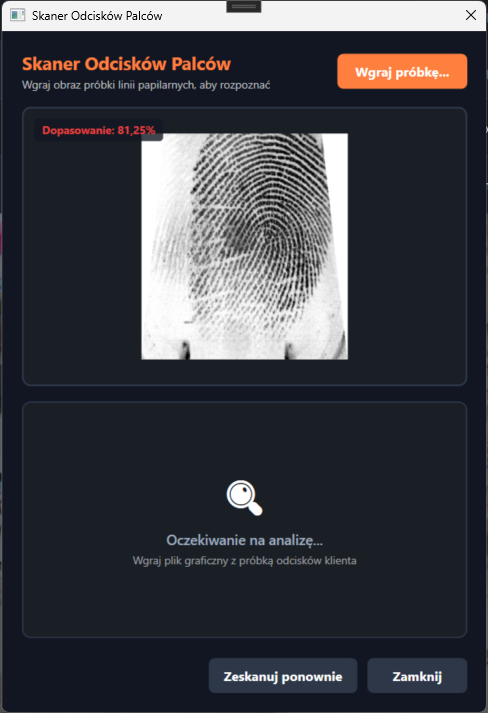
\includegraphics[width=0.45\textwidth]{figures/81error.png}
    \caption{Wynik oprogramowania podczas testów doboru progu akceptacji}
    \label{81_error}
\end{figure}

\subsection{Testy ułożenia palca}
Oprogramowanie badano również pod kątem tolerancji na różne kąty przyłożenia opuszka do skanera (rotacja i przesunięcie). Wnioski z testów pokazują, że niedbałe lub zrotowane przyłożenie palca nie pozwala na poprawne uwierzytelnienie, generując wyniki dalekie od pożądanego poziomu.


\section{Analiza bezpieczeństwa i podatność na fałszerstwa}

\subsection{Próby oszukania systemu}
W celu weryfikacji odporności systemu na intruzów, przeprowadzono testy z wykorzystaniem zupełnie obcego palca, niepowiązanego w żaden sposób z testowanym profilem. Przyłożenie niezarejestrowanego odcisku generowało wyniki prawdopodobieństwa dopasowania rzędu 45-65\%. Tak wysoki maksymalny odsetek zgodności dla błędnego dopasowania jest w głównej mierze spowodowany niewielką ilością zarejestrowanych odcisków w testowej bazie danych. Niemniej jednak, zgodnie z ustanowionym rygorystycznym progiem akceptacji na poziomie 82\%, system bez najmniejszego problemu odrzucał takie próby, gwarantując bezpieczeństwo i każdorazowo powiadamiając pracownika o braku dopasowania.

\begin{figure}[H]
    \centering
    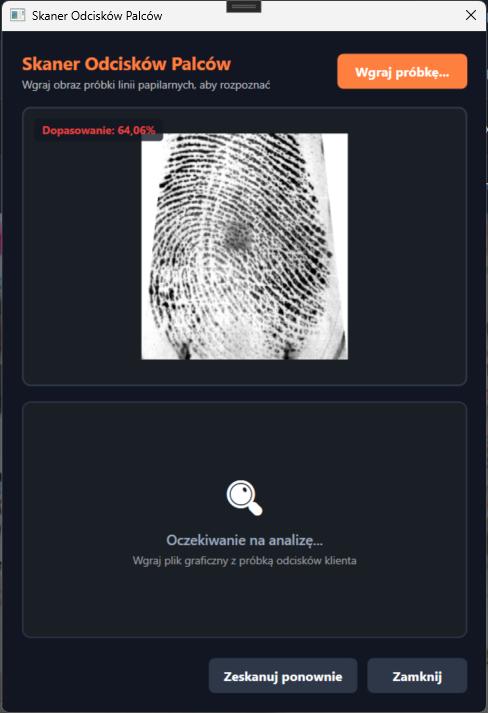
\includegraphics[width=0.45\textwidth]{figures/oszust.png}
    \caption{Przykładowy wynik oprogramowania podczas testów oszukania systemu}
    \label{oszust}
\end{figure}

\subsection{Bezpieczeństwo danych wrażliwych}
Jednokierunkowość procesu hashowania zapewnia ochronę zebranych danych biometrycznych. Wyliczony i przechowywany z obrazka 64-bitowy hash jest matematycznie niemożliwy do odwrócenia -- na jego podstawie atakujący nigdy nie wygeneruje z powrotem oryginalnego wzoru linii papilarnych. Choć aplikacja w teorii przechowuje w bazie również surowe zdjęcia w celach poglądowych dla pracowników, to mechanizm logowania jest całkowicie niezależny od nich, chroniąc obiekt przed poważnymi wyciekami.

\section{Ewaluacja i błędy identyfikacji w środowisku roboczym}
Największym wyzwaniem dla omawianego modułu okazały się uwarunkowania środowiskowe i specyfika grupy docelowej. Aplikacja Rock Gym jest przeznaczona na ściankę wspinaczkową, co w dużej mierze definiuje niezwykle trudne warunki brzegowe dla optyki urządzeń skanujących.

Osoby trenujące wspinaczkę regularnie narażają dłonie na mikrourazy. Charakteryzują się bardzo suchą skórą, częstymi przetarciami naskórka oraz korzystają z magnezji. Dodatkowym czynnikiem jest częste stosowanie po treningu kremów nawilżających. W takich "brudnych" warunkach zanieczyszczenia drastycznie obniżają jakość obrazu pozyskiwanego przez skaner. Zanieczyszczanie szkła czytnika pyłem z magnezji, zatłuszczenia z kremu prowadziłyby tylko do fałszywych odrzuceń (FRR). Rozwiązaniem tego problemu pozostaje jedynie pouczanie klientów o konieczności umycia dłoni przed skanowaniem, co pozwala na prawidłową autoryzację.
